\documentclass[a4paper, 10pt]{article}

\usepackage{setspace}
\setstretch{1.15}

\usepackage[a4paper, top=45mm, headsep=15mm, left=30mm, right=20mm, bottom=40mm]{geometry}
\usepackage{background}
\usepackage{caption}
\usepackage{float}

\usepackage{graphicx}
\graphicspath{ {./images/} }

\usepackage{titlesec}
\titlespacing*{\section}
{0pt}{22pt}{8pt}
\titlespacing*{\subsection}
{0pt}{16pt}{6pt}

\pagestyle{empty}

\backgroundsetup{
scale=1,
color=black,
opacity=1.0,
angle=0,
contents={%
    
\includegraphics[width=\paperwidth]{header+footer.pdf}
    }%
}

\usepackage[default]{opensans}
\usepackage[T1]{fontenc}
\usepackage{booktabs}

\usepackage{url}
\usepackage[all]{nowidow}

\usepackage[german]{babel}
\usepackage{csquotes}

\usepackage[dvipsnames]{xcolor}
\usepackage[colorlinks=true,colorlinks,
linkcolor=MidnightBlue,
citecolor=MidnightBlue,
urlcolor=MidnightBlue,
filecolor=blue]{hyperref}

\hypersetup{
pdftitle={Technische Anleitung - Readme},
pdfsubject={Selbstlerneinheit 12-Kanal-EKG},
pdfauthor={Eliah Lohr},
pdfkeywords={technische Anleitung, readme, Selbstlernen, EKG}
}

\usepackage[capitalise]{cleveref}

\newcommand{\warn}[1]{\textcolor{red}{#1}}
\newcommand{\code}[1]{\texttt{#1}}
\newcommand{\emoji}[1]{
    \begingroup\normalfont
    \includegraphics[height=0.8em]{emojis/#1.png}
    \endgroup
}
\newcommand{\realtilde}{{\raise.17ex\hbox{$\scriptstyle \mathtt{\sim}$}}}

% --- Tooltip box start ---
% for adjustwidth environment
\usepackage[strict]{changepage}

% for tooltips
\usepackage{framed}

% environment derived from framed.sty: see leftbar environment definition
\definecolor{tooltippipe}{HTML}{8cc020}
\definecolor{tooltipshade}{HTML}{f3fdde}

\newenvironment{tooltip}{%
\small
\vspace*{-4mm}
    \def\FrameCommand{%
    \hspace{1pt}%
    {\color{tooltippipe}\vrule width 0.7mm}%
    {\color{tooltipshade}\vrule width 1.5mm}%
    \colorbox{tooltipshade}%
    }%
    \MakeFramed{\advance\hsize-\width\FrameRestore}%
    \noindent% disable indenting first paragraph
    \begin{adjustwidth}{}{7pt}%
    \vspace{2pt}\vspace{2pt}%
}
{%
    \vspace{2pt}\end{adjustwidth}\endMakeFramed%
}
% --- Tooltip box end ---


\begin{document}

{ \Huge \noindent Technische Anleitung -- Readme} \newline
{ \LARGE \noindent Selbstlerneinheit 12-Kanal-EKG}

\subsubsection*{Zusammenfassung}
Dieses Readme umfasst die Inbetriebnahme der am \href{https://tu-dresden.de/med/mf/mitz}{Medizinisch Interprofessionellen Trainingszentrum} des Universitätsklinikum Dresden entwickelten EKG-Selbstlerneinheit für Studierende. Es beschreibt materielle und technische Voraussetzungen, ein empfohlenes räumliches Setup, Konfiguration und die Inbetriebnahme.
Für substanzielle Teile dieses Guides wird Unterstützung der Haus-IT benötigt, das Guide ist geschrieben für Ubuntu Linux.

\section{Materielle Voraussetzungen {
\includegraphics[height=0.65em]{emojis/shopping-bags.png}}}
\label{sec:prerequisites}
Zur idealen Verwendung des Projektes wird benötigt
\begin{itemize}
    \item Eine Übungspuppe mit gut tastbaren Intercostalräumen
    \item Ein 12-Kanal-EKG + Klebeelektroden
    \item Zwei USB-Kameras mit hoher Auflösung
    \item Ein PC zum Ausführen der Projektsoftware
    \item Ein Drucker, Klebeband und ein Klebestift
\end{itemize}

\subsection{USB-Kameras}
\label{ssec:cameras}
Für stabile Anwendung sind Kameras mit hoher Auflösung, 4K UHD oder höher, empfohlen. Das Originalsetup basiert auf zwei \enquote{HP 960 4K}. Das Verwenden voneinander verschiedener Kameramodelle ist meist möglich, solange die Kameras in der gleichen Bildauflösung aufnehmen.


\subsection{PC}
\label{ssec:pc-reqs}
\begin{tooltip}
    Dieser Teil sollte mit der IT-Abteilung besprochen werden\emoji{technologist}
\end{tooltip}
Der PC benötigt mind. zwei freie USB-Ports (USB 2.0+). Das Projekt wurde mit Zielplattform Ubuntu Linux (Version 24.04.1 LTS) entwickelt.

Auf dem PC muss die Umgebungsverwaltung Conda installiert sein. Aus Rechts- und Lizenzgründen sollte die über das Community-Projekt \href{https://conda-forge.org/}{Conda-Forge\emoji{link}} bereitgestellte Variante \enquote{miniconda} genutzt werden. Das Projekt wurde mit Conda-Forge Version 24.9.2 entwickelt, sollte aber auch mit anderen Versionen funktionieren. Sollte miniconda direkt in die homedirectory des Benutzeraccounts installiert werden, können der bereitgestellte Desktop-shortcut und das dazugehörige shell script direkt verwendet werden.

Nachdem conda installiert wurde, kann es im Terminal mit dem Befehl \code{conda} verwendet werden. Conda stellt isolierte Laufzeitumgebungen zur Verfügung und muss noch über das Terminal konfiguriert werden:
\begin{enumerate}
    \item Neue Umgebung erstellen: \code{conda create -n hybparc python=3.9}
    \item Neue Umgebung Aktivieren: \code{conda activate hybparc}
\end{enumerate}

\noindent Nun ist das offene Terminal auf die neue Umgebung gesetzt. Es müssen zuerst \enquote{Pip} (Python Paketmanager) und danach via Pip noch Python Pakete installiert werden. Sollte im Terminal nachgefragt werden, ob zusätzliche Abhängigkeiten (dependencies) mitinstalliert werden sollen, sollte dies mit \code{y} bestätigt werden.

\begin{enumerate}
    \item Pip installieren: \code{conda install pip}
    \item OpenCV installieren: \code{pip install opencv-contrib-python}
    \item PyQt6 installieren: \code{pip install pyqt6}
\end{enumerate}

Es sind alle dependencies des Projektes installiert.

\section{Marker}
\label{sec:ref-markers}
Zur Nutzung des Projekts werden sogenannte Arucomarker benötigt (ähnlich zu QR-Codes). Diese müssen auf Papier ausgedruckt werden (Empfehlung mind. 100g/m\textsuperscript{2}, vollweiß) und an der Übungspuppe bzw. an den Elektroden befestigt werden. Den Projektdaten liegt hierzu ein PDF bei, dieses sollte mit Skalierung 100\% ausgedruckt werden um die vorgesehenen Maße einzuhalten. Die Marker haben verschiedene Abmessungen um für Distanzunterschiede (19, 29) und Überdeckungen (15, 16) zu kompensieren.

\noindent Die mitgelieferte Konfiguration deckt ein 12-Kanal EKG ab. Es werden insgesamt 15 Marker (10 Elektroden + 5 Ausrichtungsmarker) benötigt.

\subsection{Elektrodenmarker}
\label{ssec:electrode-markers}
\begin{enumerate}
    \item Marker ausdrucken und anhand der Trennlinien ausschneiden
    \item Die Marker links, rechts und oben \enquote{trimmen}, sodass auf den drei Seiten ca. 1 bis 2 mm weiße Umrandung überbleibt.
    \item Jeden Marker von \textbf{hinten} mit einem Streifen Klebeband bekleben (Klebeseite zum Marker hin)
    \item Den Marker Kantenparallel auf ein EKG-Klebepad kleben, sodass der Mittelpunk des Markers der oberen Kante des Befestigungsclips des Pads ca. vier bis fünf mm übersteht.
    \item Nun den unteren Teil des Markers zurechtstutzen.
    \item Den Marker mithilfe des Pad-Clips an die Elektrode anstecken, und so weit nach hinten schieben, dass bei Benutzung des Setups Platz für das eigentliche Pad ist.
\end{enumerate}

Angestrebtes Endergebnis:
\begin{figure}[H]
    \centering
    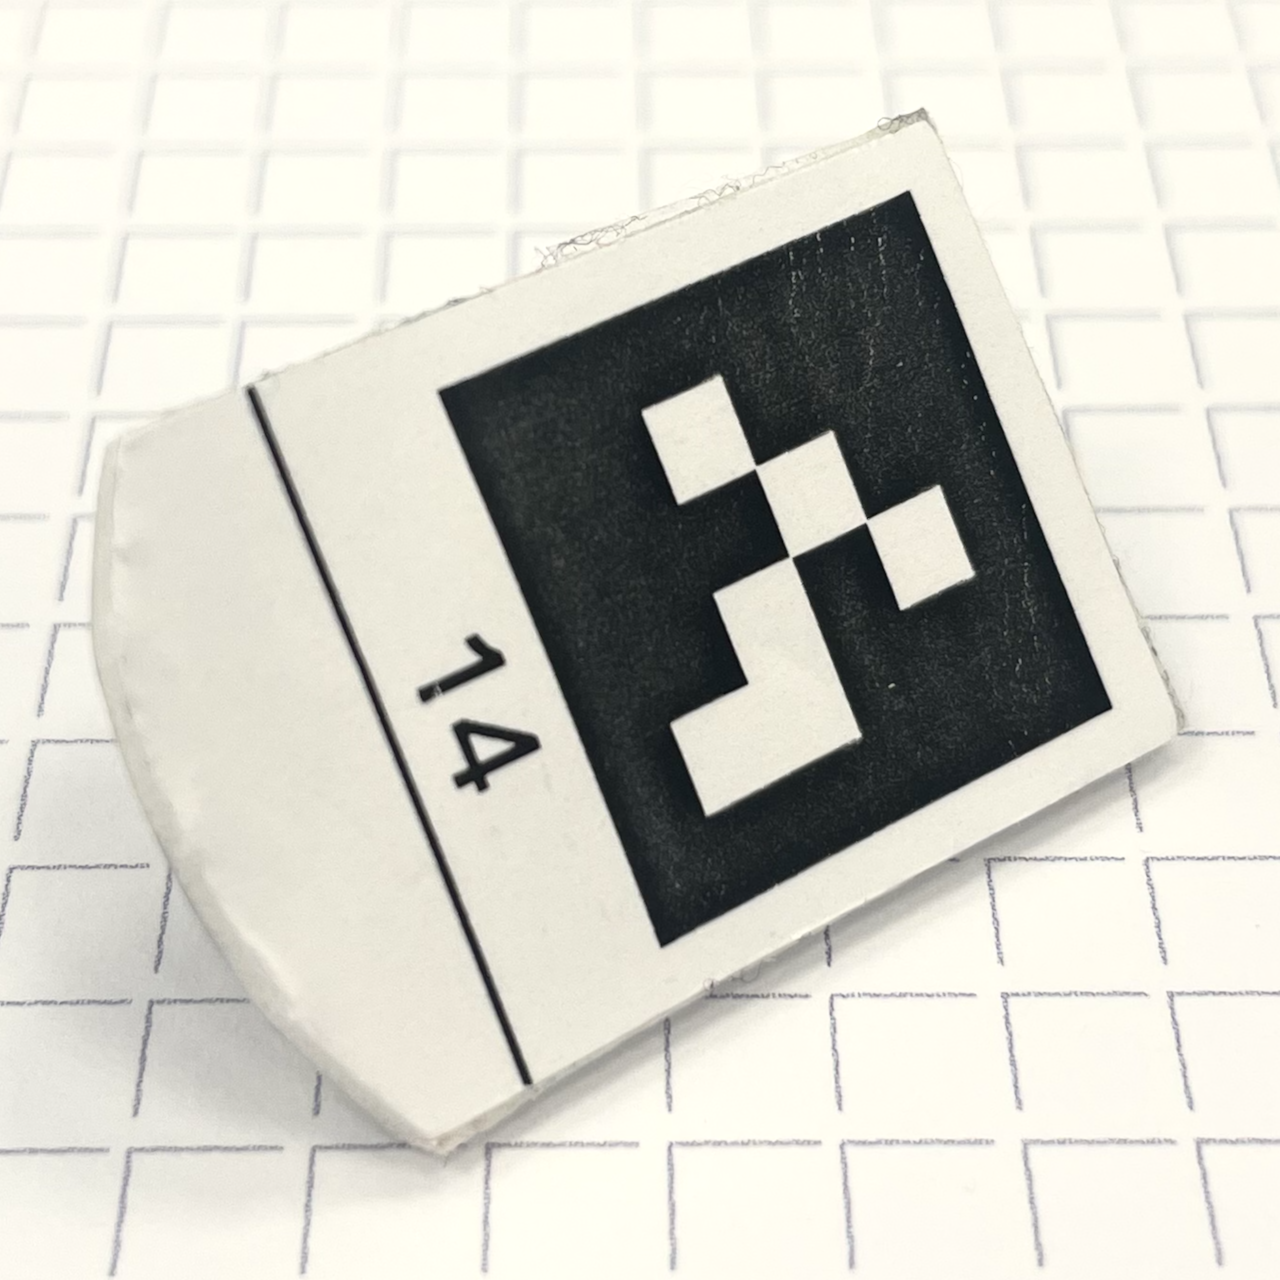
\includegraphics[width=2.5cm]{marker-front.png}
    \hspace*{5mm}
    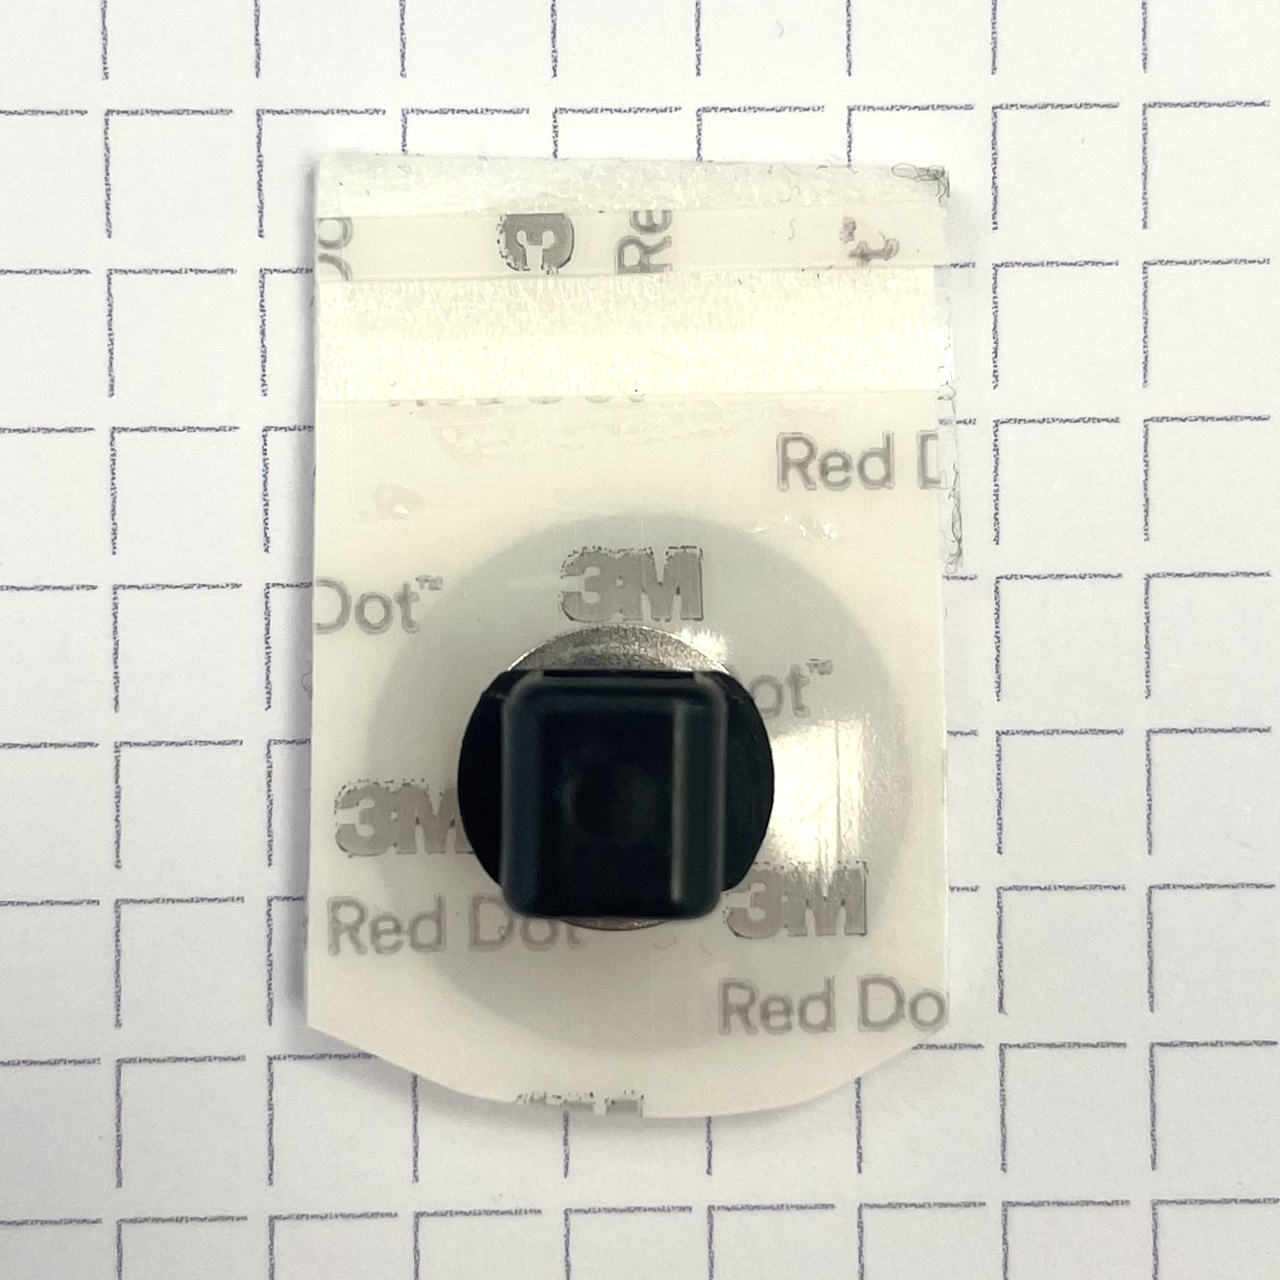
\includegraphics[width=2.5cm]{marker-back.png}
    \hspace*{5mm}
    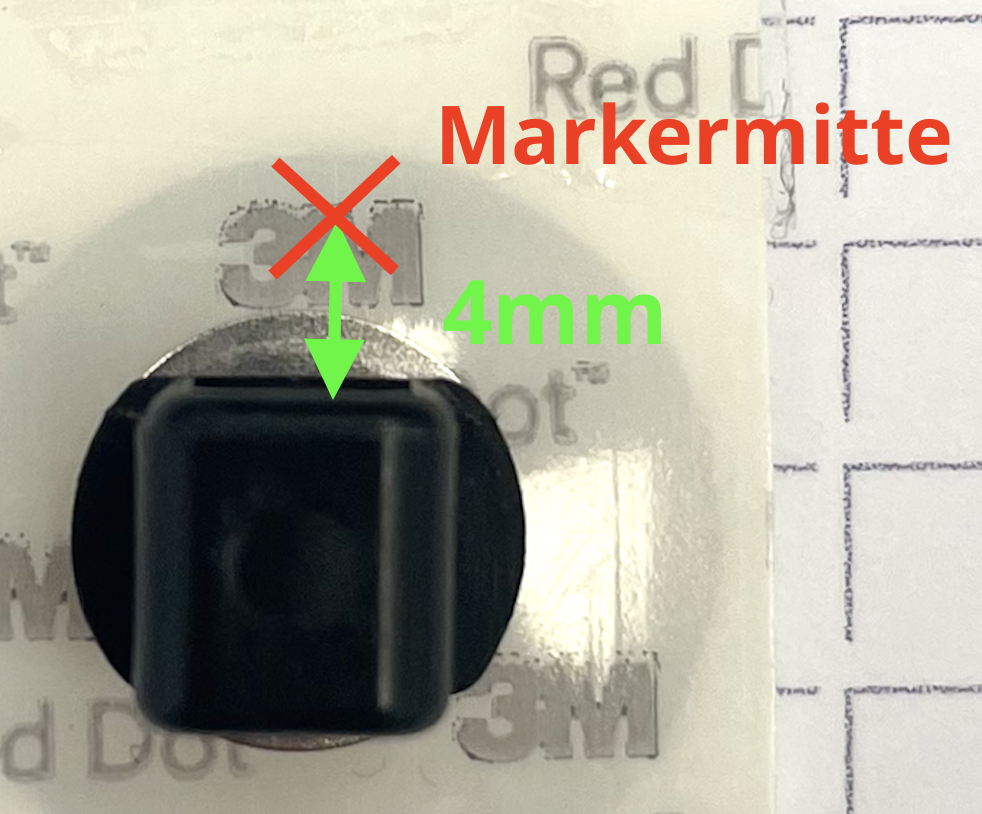
\includegraphics[width=2.5cm]{marker-back-zoomed.png}
    \hspace*{5mm}
    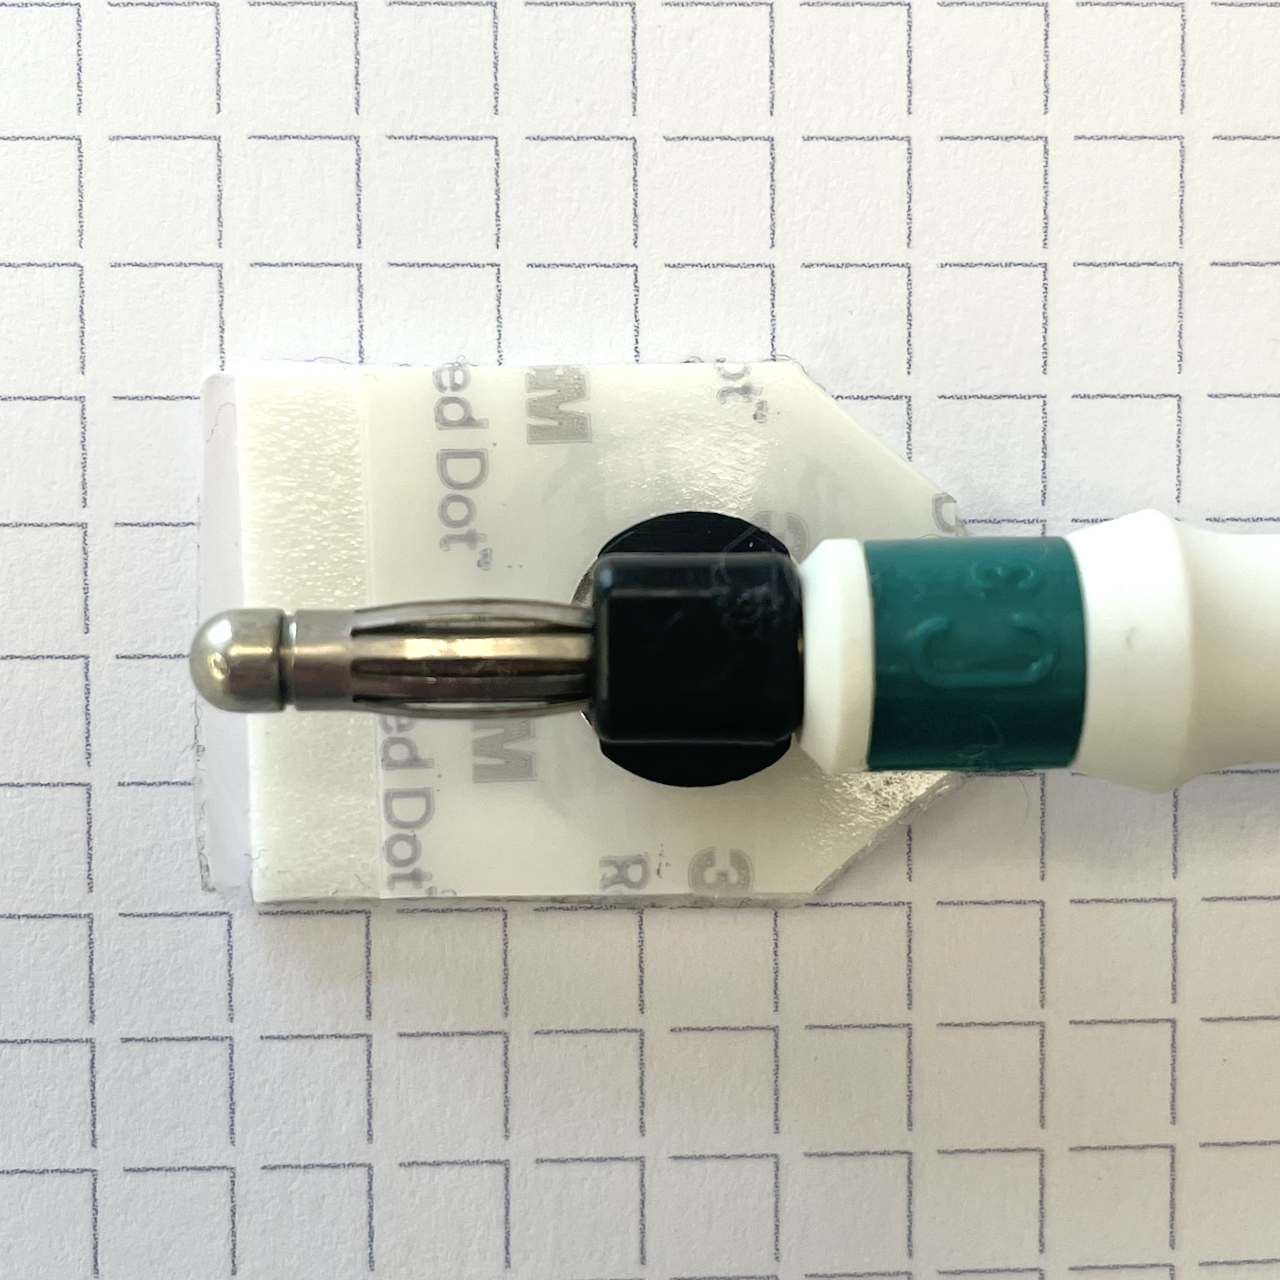
\includegraphics[width=2.5cm]{marker-attatched.png}
\end{figure}

\subsection{Ausrichtungsmarker}
\label{ssec:reference-markers}
Alle Ausrichtungsmarker müssen möglichst flach auf der Puppe angebracht werden. Es ist wichtig, dass sie unbeweglich sind und bleiben, sie dürfen nicht verdeckt werden.

\subsection{Positionierung}
\label{sssec:marker-positioning}
\begin{tooltip}
    Dieser Teil ist relevant, wenn die mitgelieferten Lagedaten verwendet werden sollen\emoji{package}
\end{tooltip}

Die Marker müssen ihrer Nummer nach an den zugehörigen Elektroden angebracht werden:
\begin{table}[H]
    \centering
    \begin{tabular}{p{11mm}| p{9.5mm} p{9.5mm} p{9.5mm} p{9.5mm} p{9.5mm} p{9.5mm} p{9.5mm} p{9.5mm} p{9.5mm} p{9.5mm}}
        Nr.  & 11  & 12  & 13  & 14 & 15 & 16 & 21 & 31 & 41  & 51 \\
        Name & V1  & V2  & V3  & V4 & V5 & V6 & Rot & Gelb & Schw. & Grün \\
    \end{tabular}
\end{table}

\noindent Um die Position der Elektroden zu bestimmen, müssen die Ausrichtungsmarker auf der Puppe angebracht werden. Diese sind entsprechend zugeordnet:
\begin{table}[H]
    \centering
    \begin{tabular}{p{10.5mm}| p{10.5mm} p{10.5mm} p{10.5mm} p{10.5mm} p{10.5mm}}
        Nr.  & 19    & 29    & 39    & 49    & 59 \\
        Name & Brust & Arm R & Arm L & Fuß R & Fuß L \\
    \end{tabular}
\end{table}

\noindent Der Brust-Ausrichtungsmarker (Nummer 19) sollte dabei mit der oberen Kante auf Höhe der zweiten echten Rippe angebracht werden, sodass der Marker selbst innerhalb des zweiten ICR liegt.
\begin{figure}[H]
    \centering
    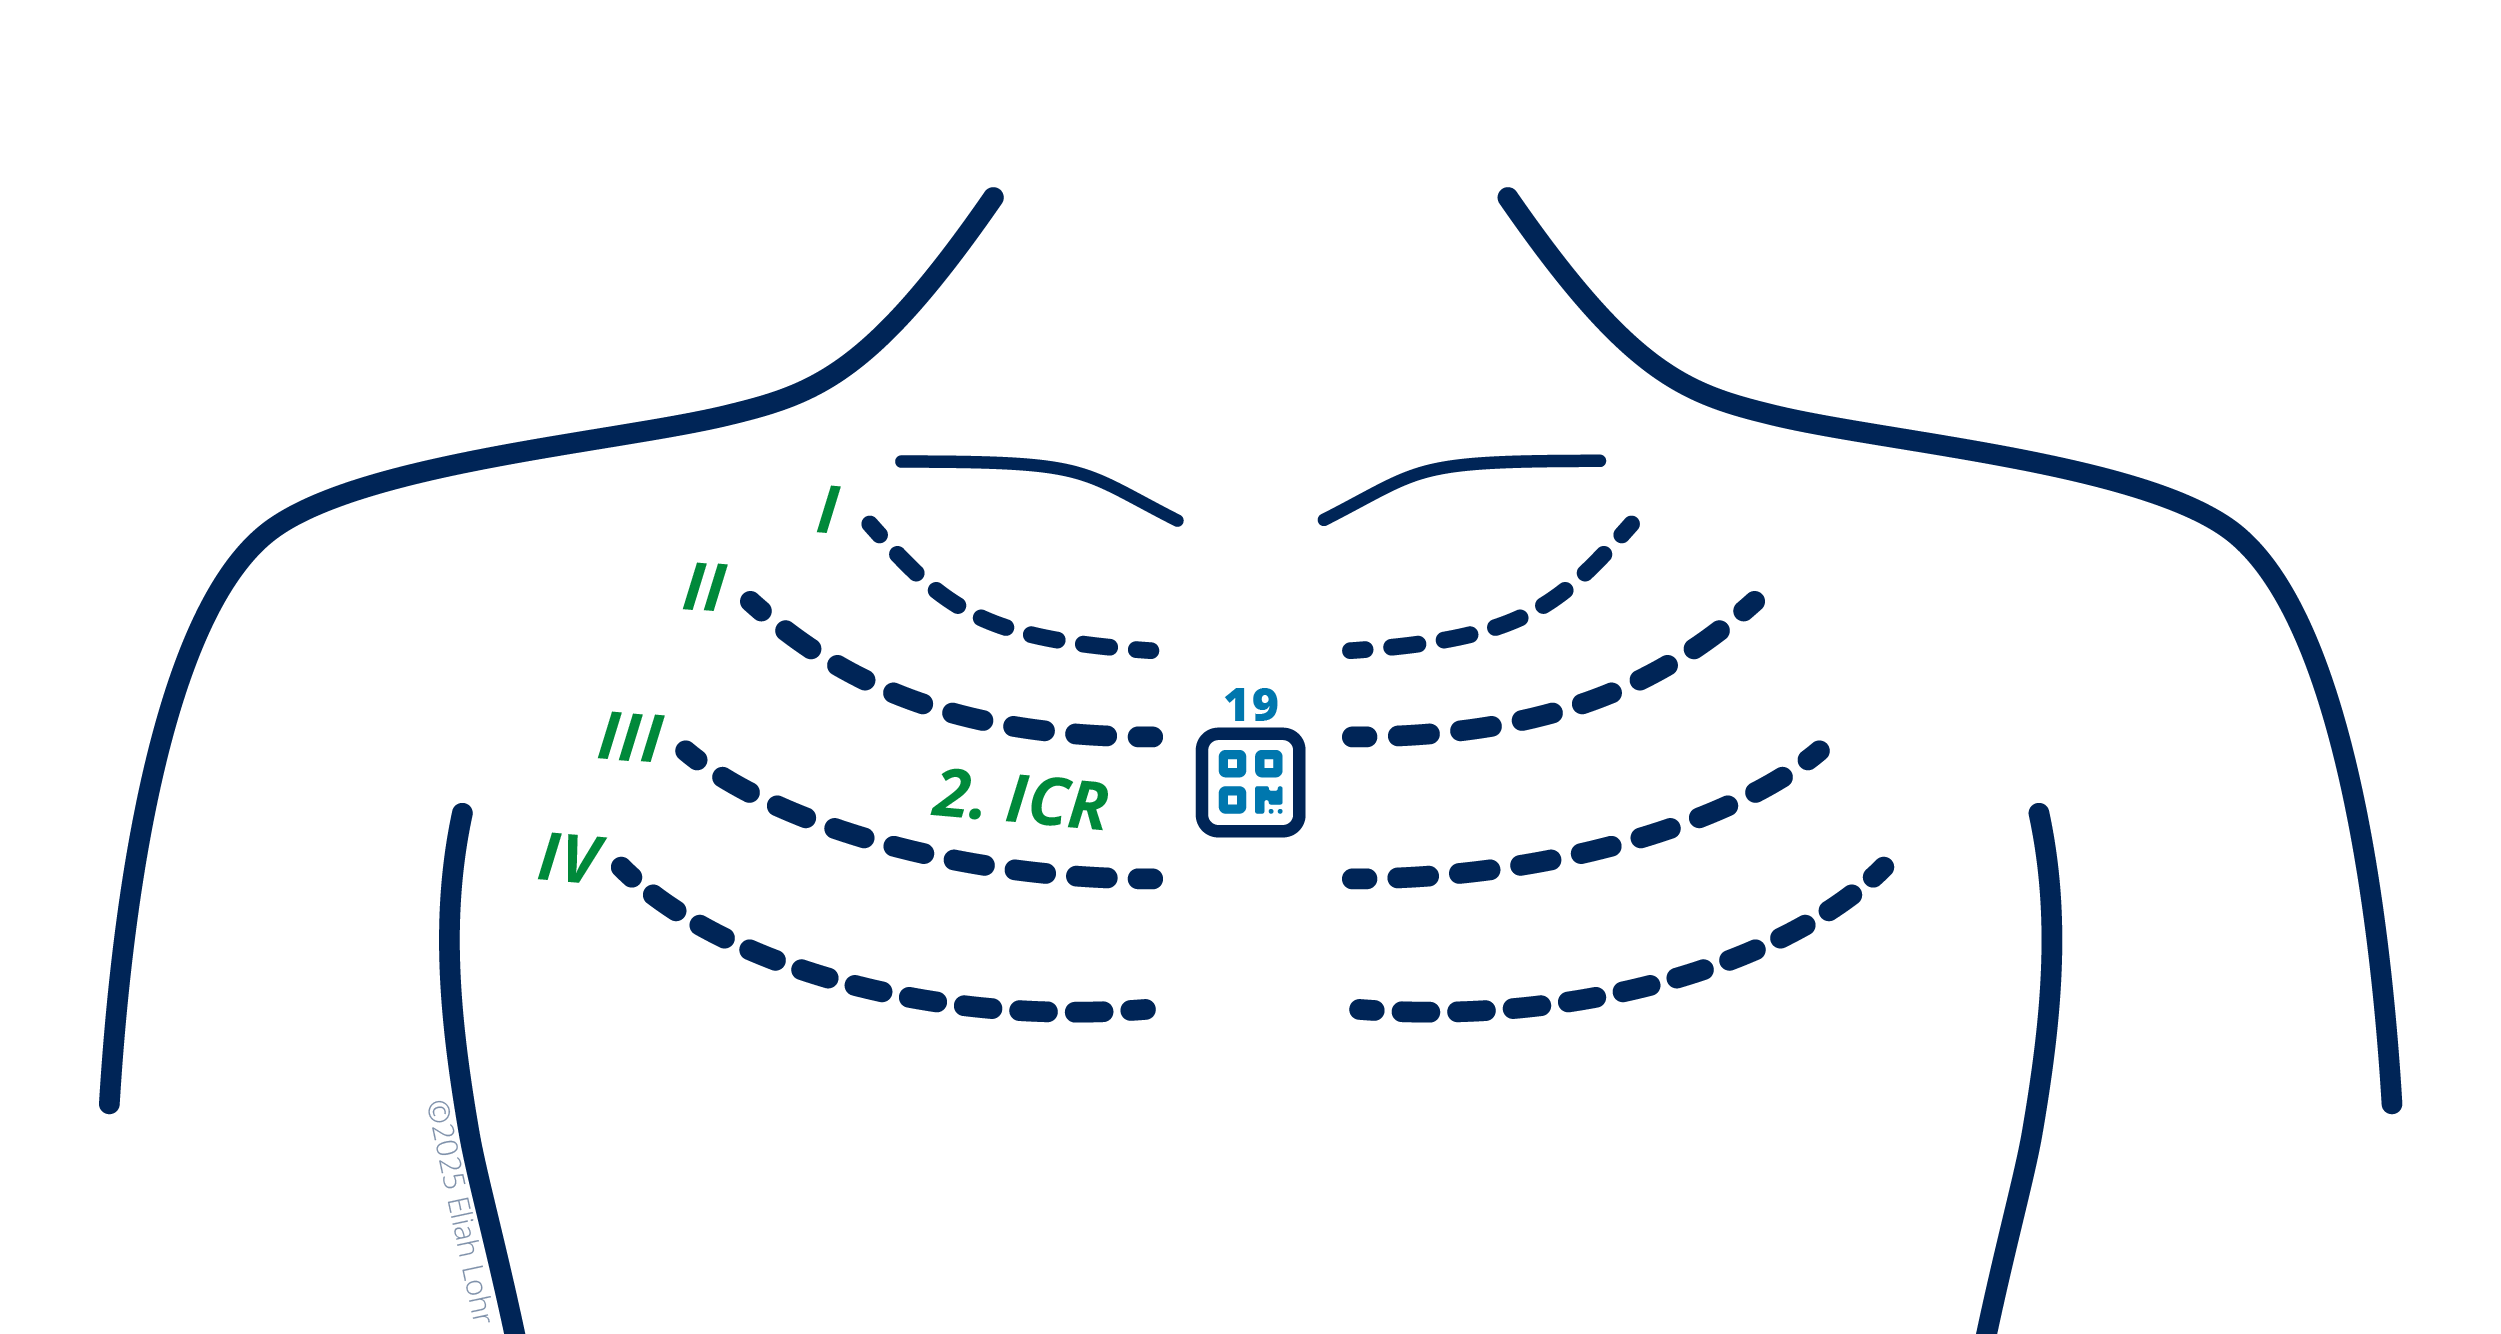
\includegraphics[width=10.5cm]{placement-torso.png}\\
\end{figure}

\noindent Die Ausrichtungsmarker der Arme müssen etwa acht cm proximal vom Handgelenk aus angebracht werden. Die Marker der Beine etwa 15 cm proximal vom Knöchel aus gesehen.

\section{Physisches Setup 
\includegraphics[height=0.65em]{emojis/hammer-and-wrench.png}}
\label{sec:physical-setup}
\begin{tooltip}
    Dieses Kapitel bezieht sich explizit auf das im MITZ erprobte Setup\emoji{index-pointing-up}
\end{tooltip}
Die Übungspuppe sollte auf einer Liege platziert werden. Die Höheneinstellung der Liege ist frei wählbar, solange die entsprechenden Parameter gewahrt werden:

\begin{figure}[H]
    \centering
    \begin{minipage}[c]{0.475\linewidth}
        \centering
        \captionsetup{labelformat=empty}
        \caption{\textit{Draufsicht} \hspace*{10mm}}
        \vspace*{-4mm}
        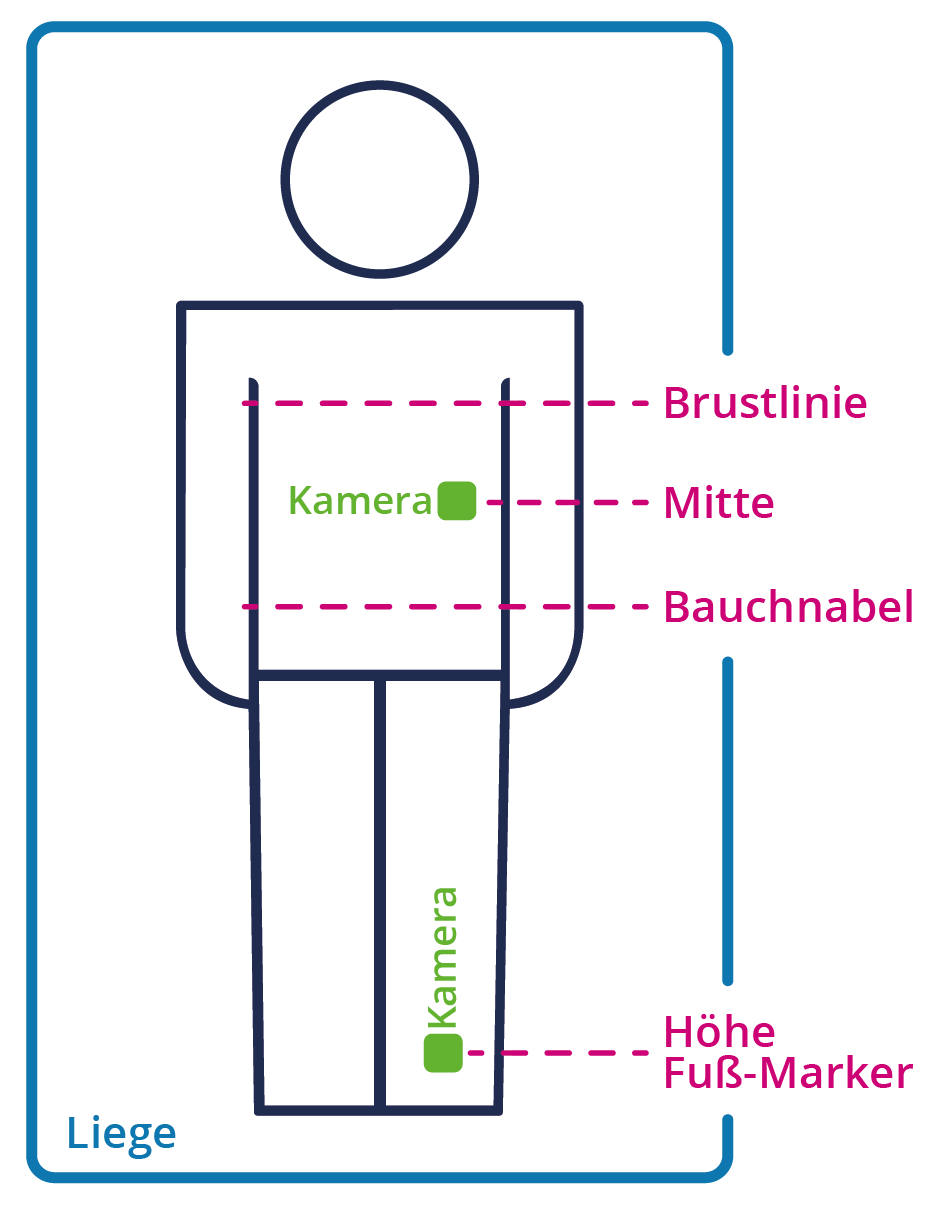
\includegraphics[width=60mm]{cam-placements_topview.png}
    \end{minipage}
    \hspace*{-4mm}
    \begin{minipage}[c]{0.5\linewidth}
        \centering
        \captionsetup{labelformat=empty}

        \caption{\textit{Torso}}
        \vspace*{-6mm}
        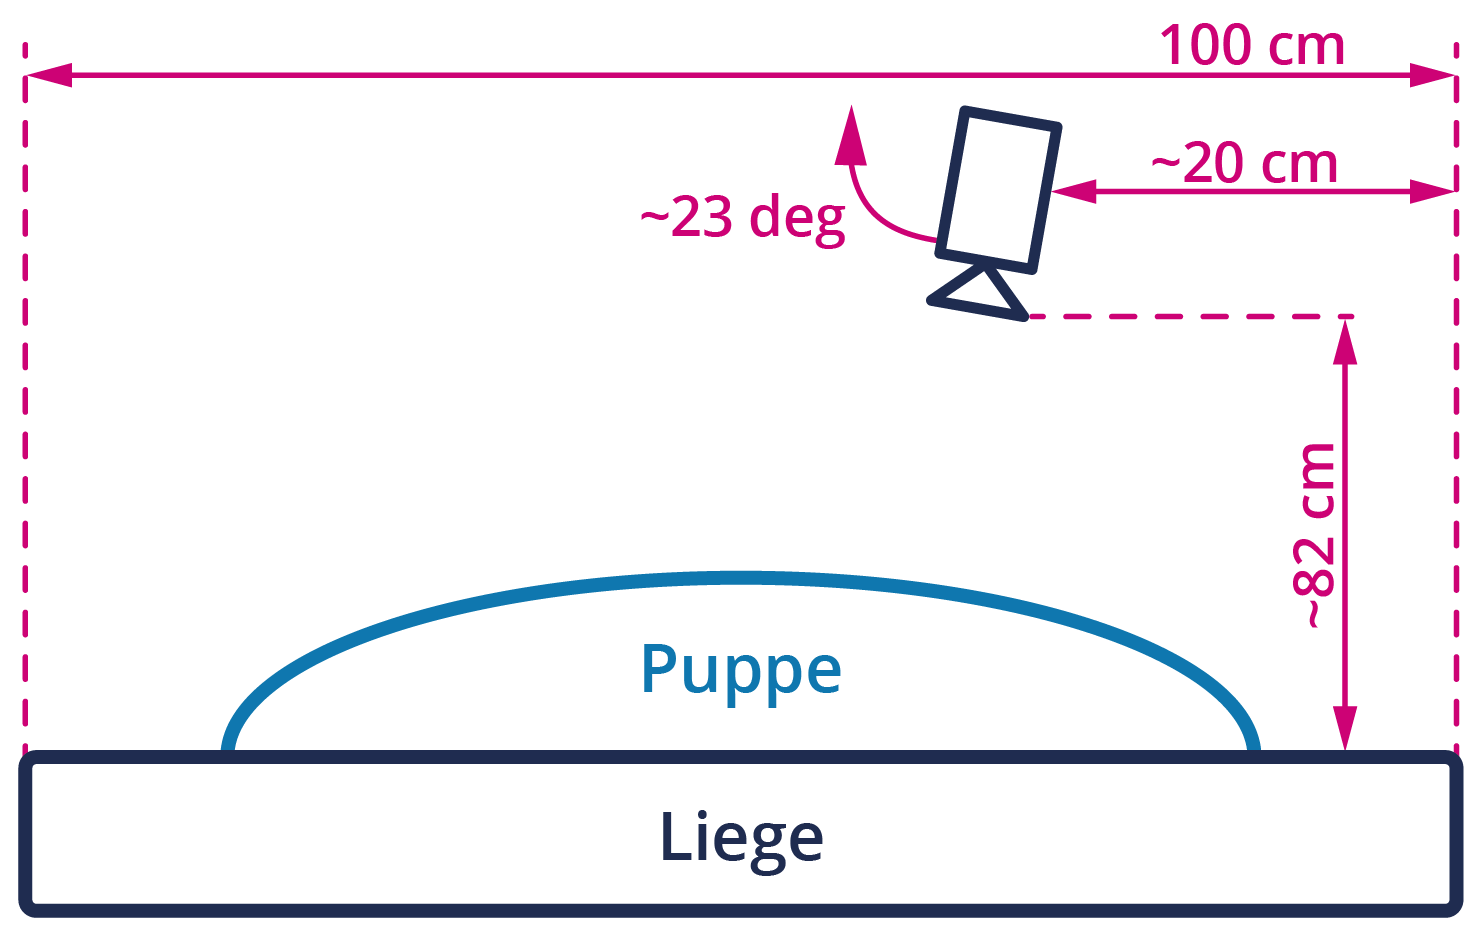
\includegraphics[width=70mm]{cam-placements_torso.png}

        \vspace*{4mm}

        \caption{\textit{Beine}}
        \vspace*{-6mm}
        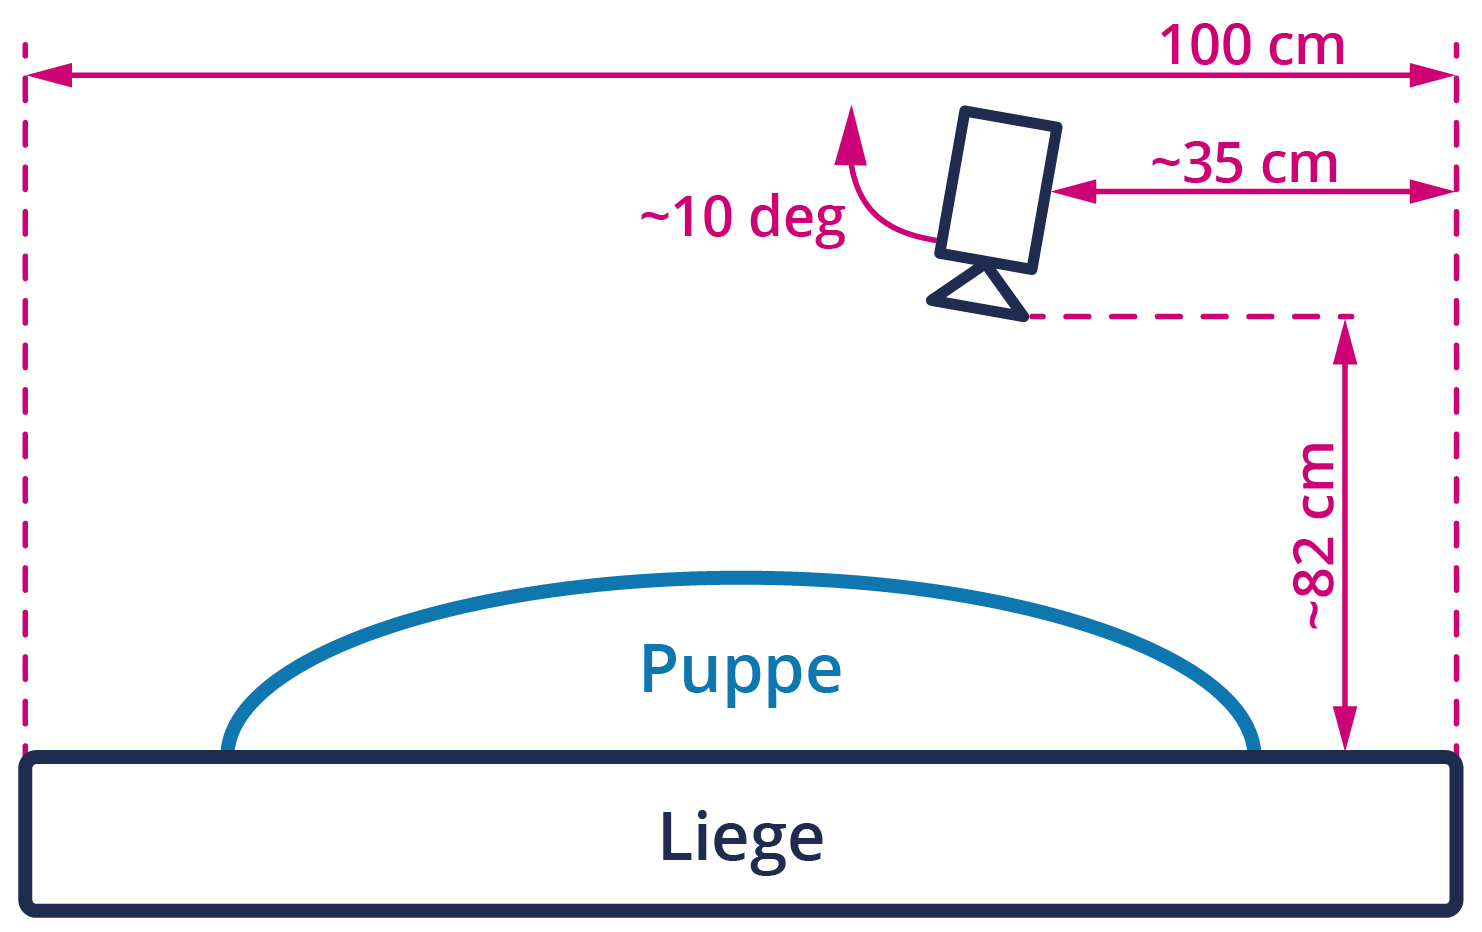
\includegraphics[width=70mm]{cam-placements_legs.png}
    \end{minipage}
\end{figure}

\noindent Für die beiden Kameras empfiehlt es sich, eine stabile und beständige Befestigungsgrundlage zu finden, welche dem anstoßen von Nutzenden widerstehen kann; sonst muss die Integrität der Kameraausrichtungen regelmäßig mithilfe von ArucoRoi (siehe \ref{ssec:configure-configuration}) nachkontrolliert werden.

\section{Projekinstallation, Konfiguration 
\includegraphics[height=0.65em]{emojis/gear.png}}
\label{sec:installation-configuration}
\begin{tooltip}
    Dieser Abschnitt sollte mit der IT-Abteilung besprochen werden\emoji{technologist}
\end{tooltip}
Es ist empfohlen, einen vorgefertigten Release von \href{https://www.twillo.de/edu-sharing/components/render/1345111e-baf1-4023-b27e-66bcd533de3a}{Twillo\emoji{link}} herunterzuladen. Bei Bedarf steht der aktuelle Sourcecode auf \href{https://github.com/leloomi/hybparc_aruco}{GitHub\emoji{link}} verfügbar. Falls der in \ref{ssec:pc-reqs} angebotene Desktop-shortcut und sein shell-Script verwendet werden sollen, muss das Projekt in der homedirectory im Ordner \code{repos} installiert werden (Gesamtpfad \code{\realtilde/repos/hybparc\_aruco/}).

Sollten die verwendeten Kameras die \textbf{exakt} gleiche Auflösung (3840x2160) wie die des Originalsetups haben, und MJPEG unterstützen, sollte\textsuperscript{\tiny TM} das Projekt (unter Ubuntu Linux) nun ohne Probleme funktionieren. 

\subsection{Kamera-IDs}
\label{ssec:cam-indices}
Potentiell müssen die interface IDs angepasst werden, diese können mit den v4l2 command line tools (müssen potenziell nachinstalliert werden) ausgelesen werden: \code{v4l2-ctl --list-devices}. Die Konfigurations-\enquote{Reihenfolge} der Kameras (Unterkörper vs. Oberkörper) spielt keine Rolle. Die entsprechenden IDs müssen in der Datei \code{main.py} angepasst werden:
\begin{figure}[H]
    \centering
    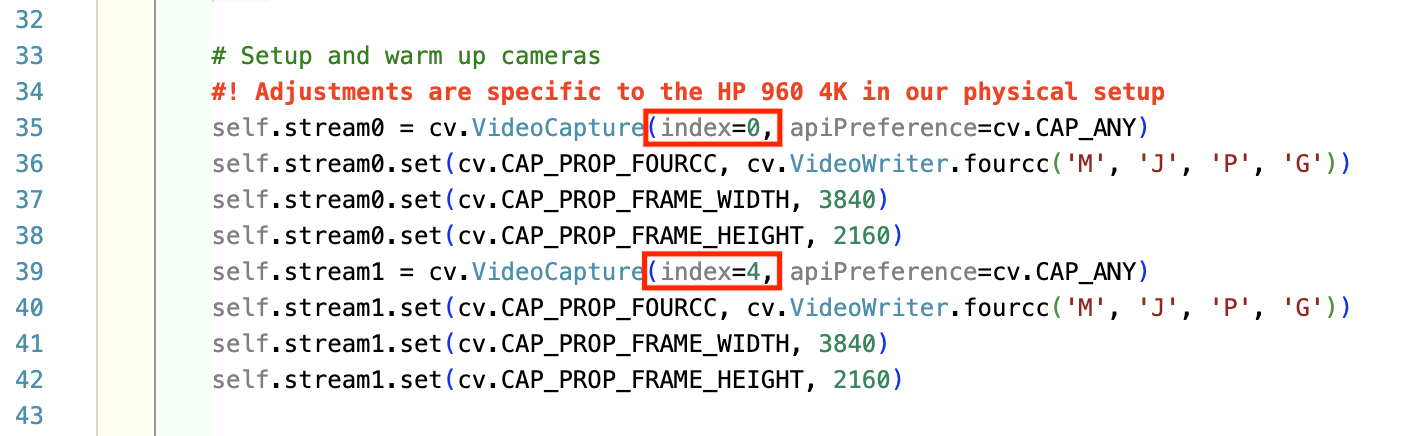
\includegraphics[width=10.5cm]{camera-indices.png}
\end{figure}

\subsection{Andere Auflösung}
\label{ssec:custom-resolution}
Bei anderen Auflösungen müssen im Code unter \code{/hybparc\_aruco/main.py} fast zu Beginn der \code{\_\_init\_\_} Funktion die entsprechenden Parameter angepasst werden:
\begin{figure}[H]
    \centering
    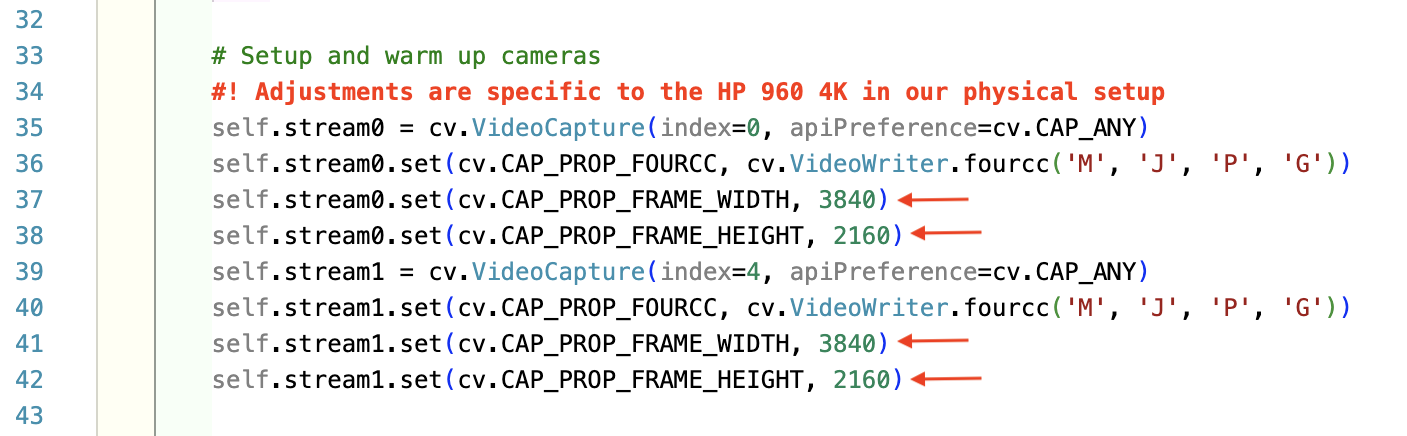
\includegraphics[width=10.5cm]{resolution.png}
\end{figure}

\subsection{Kein MJPEG 
\includegraphics[height=0.75em]{emojis/open-mouth.png}}
\label{ssec:the-mjpeg-problem}
Das Projekt wurde ausschließlich mit MJPEG getestet. Bei unbedingtem Bedarf kann jedoch probiert werden, das Format umzustellen. Die unterstützten Formate einer Kamera bzw. des Interfaces mit der Nr. X können via \code{v4l2-ctl -d /dev/videoX --list-formats-ext} ausgelesen werden. Der entsprechende Codec muss im \href{https://fourcc.org/codecs.php}{FourCC Format\emoji{link}} unter \code{/hybparc\_aruco/main.py} fast zu Beginn der \code{\_\_init\_\_} Funktion angepasst werden:
\begin{figure}[H]
    \centering
    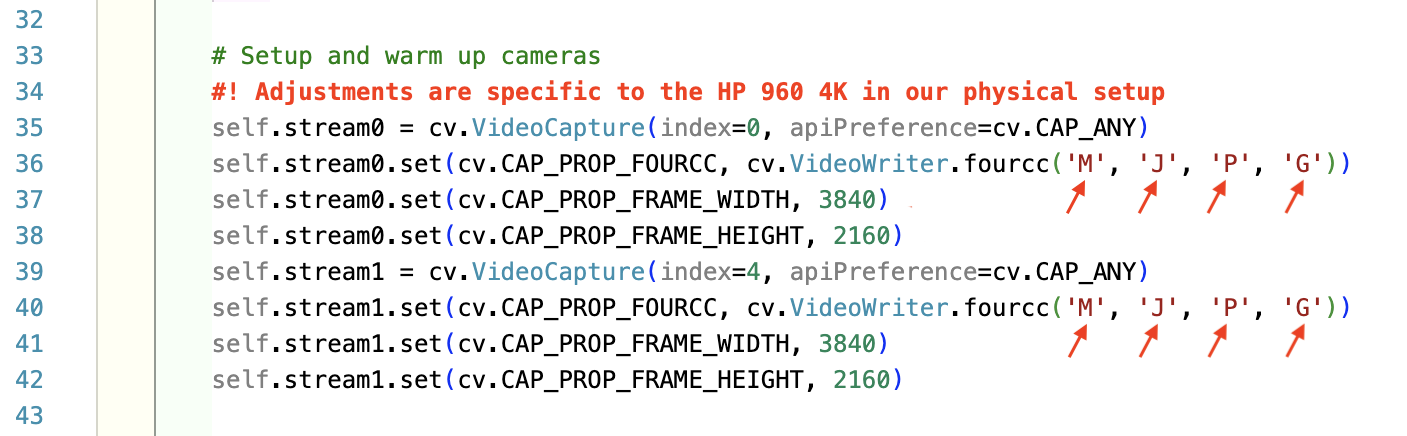
\includegraphics[width=10.5cm]{fourcc.png}
\end{figure}

\subsection{Desktop shortcut 
\includegraphics[height=0.75em]{emojis/sparkles.png}}
\label{ssec:desktop-drip}
Um Nutzenden einfachen Zugang zu ermöglichen, empfiehlt sich die Einrichtung eines Desktop-shortcuts. Da das Projekt in einem Conda-environment läuft sind dazu mehrere Schritte empfohlen. Empfohlenerweise liegt auf dem Desktop eine Verknüpfung \code{starte-ekg.desktop} mit dem Inhalt
\begin{verbatim}
    [Desktop Entry]
    Name=Starte EKG
    Comment=MITZ Selbstlerneinheit
    Exec=/home/selbstlern/repos/starte-ekg.sh
    Terminal=false
    Type=Application
\end{verbatim}
{\footnotesize(das Projekt liegt hier in der homedirectory des Nutzers \enquote{selbstlern}, im Ordner \code{/repos/})}\\
Die durch den shortcut aufgerufene \code{starte-ekg.sh} enthält lediglich
\begin{verbatim}
    cd ~/repos/hybparc_aruco
    ~/miniforge3/envs/hybparc/bin/python3 main.py
\end{verbatim}
wobei Zeile 1 den Ausführungsort auf den Projektordner setzt, und Zeile 2 zum ausführen der \code{main.py} den direkten Pfad der python-executable nutzt, die in das hybparc conda-environment installiert ist. So kann erreicht werden, dass Nutzende ausschließlich das user interface sehen.

Die beiden Zeilen können \emph{nicht} vereinigt werden! Der change directoy\textsuperscript{(cd)} Befehl ist nötig um das Projekt in seinem Ordner auszuführen, sonst zerbrechen Abhängigkeiten. Um das shellscript tatsächlich ausführbar zu machen, muss es via Terminal mit dem Befehl \code{chmod +x starte-ekg.sh} \enquote{behandelt} werden.

\subsection{Auswertung konfigurieren}
\label{ssec:configure-configuration}
\begin{tooltip}
    Dieser Schritt ist auch beim Verwenden der Vorgefertigten Markerkonfiguration notwendig\emoji{head-shaking-vertically}
\end{tooltip}
Je nach Unterschieden im Setup (Kameraauflösung, Kameradistanzen, Kamerawinkel) müssen die vorhandenen Lagekonfigurationen im File \code{mitz-ekg-config.json} angepasst werden. Die Konfiguration liegt im JSON Format vor und strukturiert sich wie folgt:
\begin{figure}[H]
    \centering
    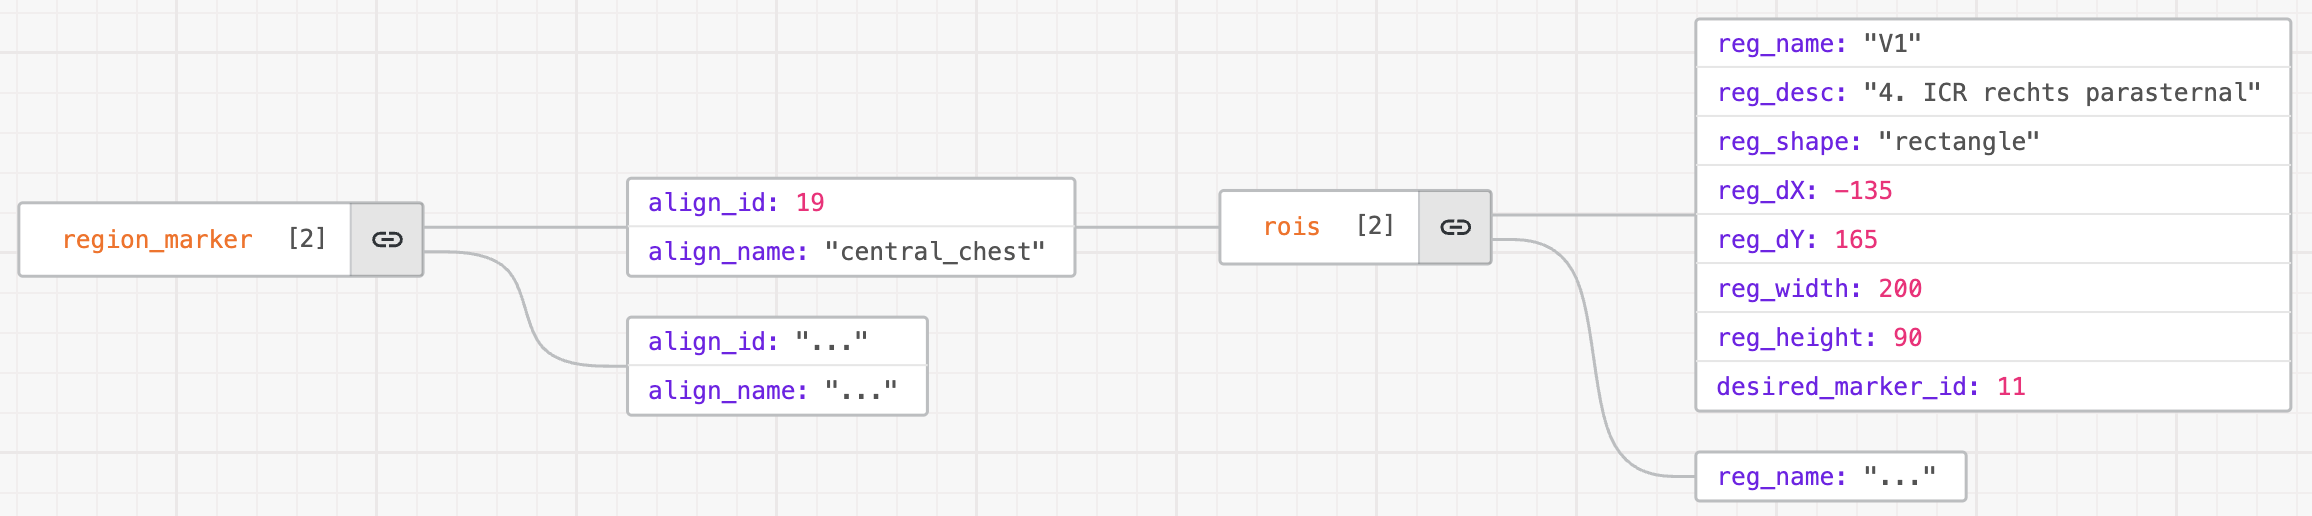
\includegraphics[width=13.5cm]{json-tree.png}
\end{figure}

\noindent Wobei jeder Eintrag der Arrays \code{rois} jeweils einen \enquote{Elektrodenbereich} definiert:
\begin{figure}[H]
    \centering
    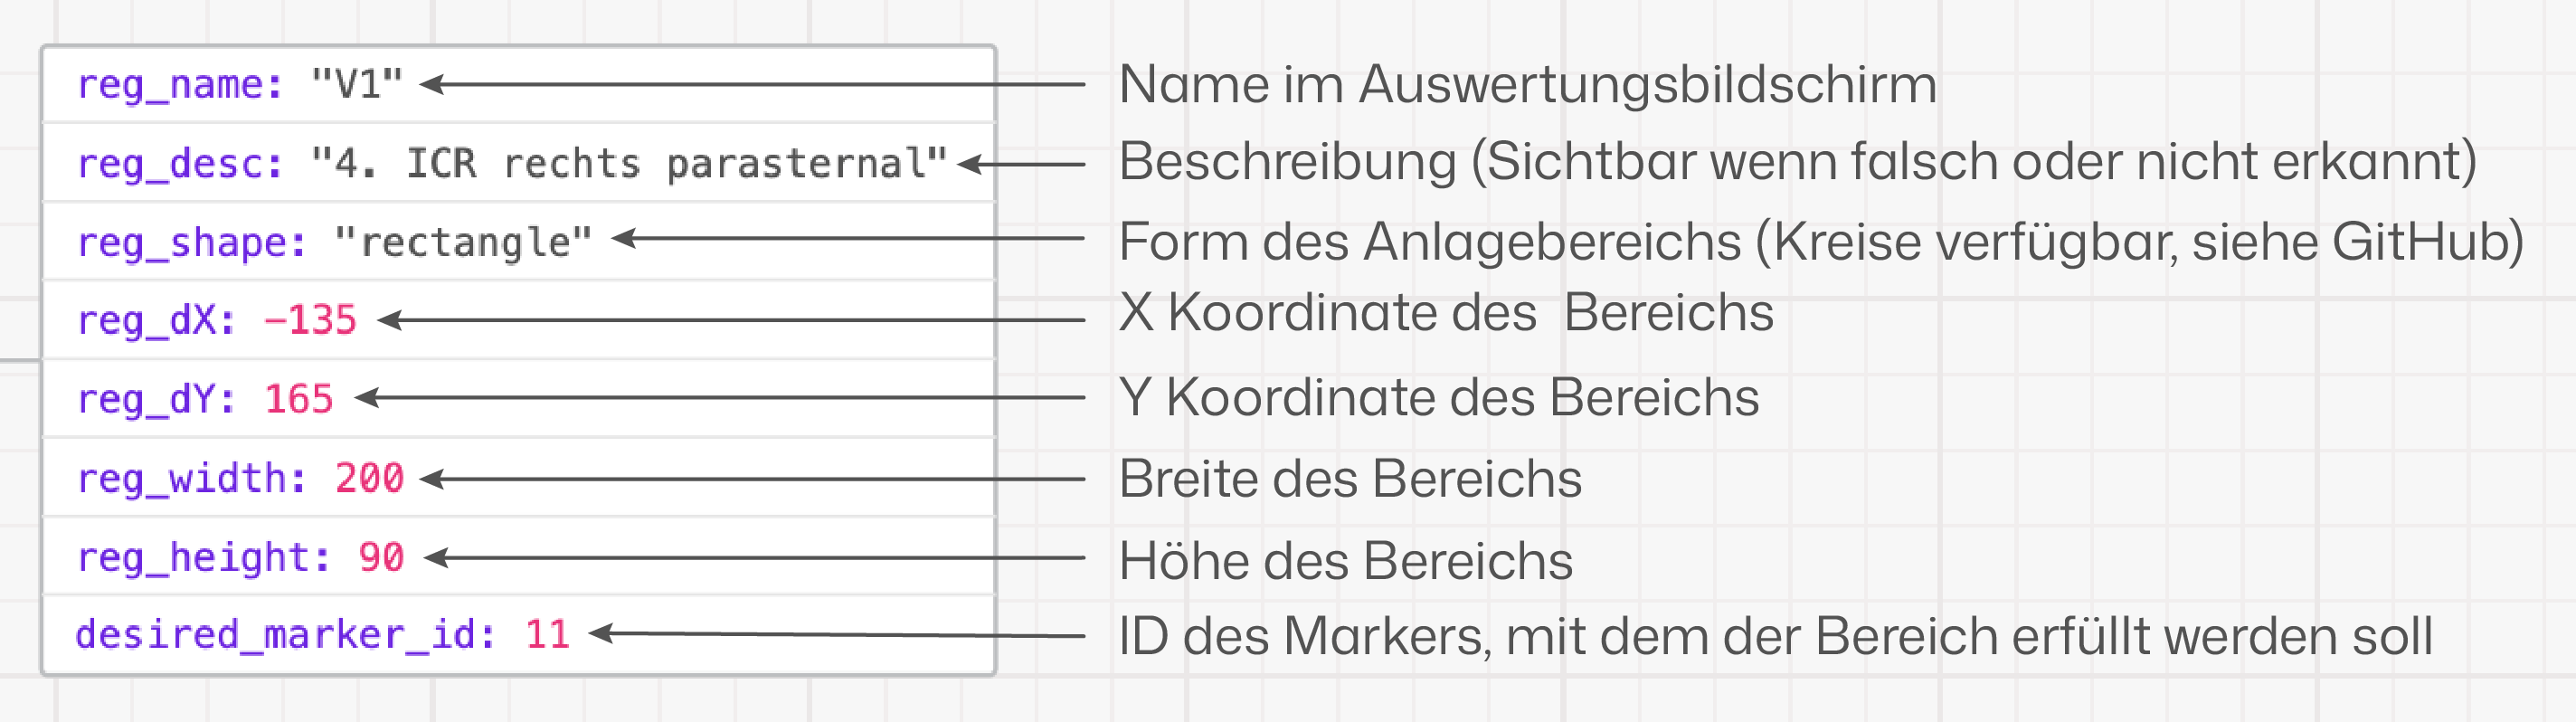
\includegraphics[width=10.5cm]{json-explainer.png}
\end{figure}

\noindent Die Positionierungen und Größen aller Bereiche müssen vor Verwendung des Projektes mit für medizinischem Personal überprüft und Fehler korrigiert werden. Um die Konfigurationen live anzupassen, empfiehlt es sich das Tool \href{https://github.com/leloomi/arucoroi}{ArucoRoi\emoji{link}} zu verwenden; es liegt dem Projekt bei und ermöglicht Live-Anpassung der Konfigurationen. Es muss über das Terminal im selben Conda-environment verwendet werden wie das Hauptprojekt (\code{conda activate hybparc}) und kann mit \code{python example.py} im Ordner \code{ArucoRoi} ausgeführt werden. 

Wenn das in diesem Ordner liegende Config-File verändert gespeichert wird, werden auch die Bereiche auch im Live-View aktualisiert. Um die Config mit der anderen Kamera zu testen muss in der \code{example.py}, Zeile 8, die Kamera ID geändert und ArucoRoi neugestartet werden (siehe \ref{ssec:cam-indices}). Die software kann mit \code{q} geschlossen werden.

Die fertig angepasste Konfiguration muss abschließend noch in den \code{hybparc\_aruco} Ordner kopiert werden um die veraltete zu ersetzen.
\section{
\includegraphics[height=0.65em]{emojis/police-light.png} Troubleshooting 
\includegraphics[height=0.65em]{emojis/police-light.png}}
\label{sec:troubleshooting}

Um das Projekt über das Terminal zu starten, oder um Änderungen am conda environment vorzunehmen, muss das environment bei jedem Terminal neustart wieder aktiviert werden (\code{conda activate hybparc}).

\paragraph{OpenCV Package Type}
Das Guide empfiehlt \code{opencv-contrib-python} zu installieren. Dies ist eine Ubuntu Linux spezifische Empfehlung. Sollte das Projekt unter MacOS und Windows verwendet werden empfiehlt sich das Package \code{opencv-python}.

\paragraph{Kontrollbilder}
Zur Kontrolle können die für die Auswertung genutzten Bilder abgespeichert werden. Hierfür muss im Projektordner einfach ein Ordner \enquote{results} erstellt werden.
\\
{\footnotesize 
\includegraphics[height=0.6em]{emojis/warning.png} Nach Kontrolle Ordner löschen, die Bilder sind unkomprimiert und damit sehr groß! 
\includegraphics[height=0.6em]{emojis/warning.png}}

\section{Known Issues 
\includegraphics[height=0.65em]{emojis/pensive.png}}
\label{sec:known-issues}
\paragraph{Abhängigkeit von Lichtverhältnissen} Da die Software Kamerabasiert arbeitet, ist sie stark abhängig von den Lichtverhältnissen. Die besten Ergebnisse lassen sich erzielen, wenn Tageslicht vom Raum ausgeschlossen wird (Rollo) und dafür ausreichen top-down Beleuchtung durch das Deckenlicht erreicht wird.

\paragraph{Crash noch vor der Auswertung} Leider sind die Zeiten mit denen  Kameras für die Software verfügbar sind abhängig vom Betriebssystem, (gefühlt) der Raumtemperatur(?), dem PC und dessen Tagesstimmung usw. Es kann also vorkommen, dass die Software abstürzt, sollte \enquote{zu schnell} auf auswerten gedrückt werden. Hier muss die Software einfach neugestartet werden und vor dem Auswerten 15-30s gewartet werden. Sobald einmal eine Auswertung vorgenommen wurde, sind die Kameras an die Software gebunden und solche crashes treten nicht mehr auf.

\paragraph{Langsamer Autofokus}
Leider sind die Auswertungen davon abhängig, dass der Autofokus der Kameras gut funktioniert. Hat eine Kamera einen schlechten Tag, so kann es sein, dass ein zweites Mal ausgewertet werden muss.

\section{Feedback}
In diesem Guide nicht aufgeführte Fehler können gern via \href{https://github.com/LeLoomi/hybparc_aruco/issues}{GitHub Issues\emoji{link}} gemeldet werden, ebenso Verbesserungsvorschläge für dieses Readme.


% upper end of document footer
\begin{figure}[b]
    \begin{flushleft}
        \hspace*{7.4mm}
        {\footnotesize Stand \today}
    \end{flushleft}
    \vspace{-3.3mm}
    \centering
    
\includegraphics[width=14.61cm]{funding+license.png}
\end{figure}

\end{document}